 \section{Concept Drift Components}
\label{sec:background_concept_drift_components}
Conventional machine learning involves prediction and training, but learning under the concept drift paradigm introduces three additional steps: concept drift detection, drift understanding, and drift adaptation \ref{fig:concept-drift-components}. Concept drift detection identifies changes in the data distribution, pinpointing when and where drift occurs. Drift understanding analyzes the timing, duration, and location of drift, offering critical insights for the adaptation step. Adaptation, or reaction, involves updating models in response to detected drift. Approaches for drift adaptation include Simple Retraining, Ensemble Retraining, and Model Adjusting. Drift detection methods vary, with some using constant chunk lengths and others employing variable lengths. Drift understanding helps inform decisions on whether to retrain a model from scratch or adjust the existing one, based on the severity of the drift as shown in Fig. \ref{fig:concept-drift-understanding}.
\vspace{-3mm}

\begin{figure}[!ht]
    \centering
    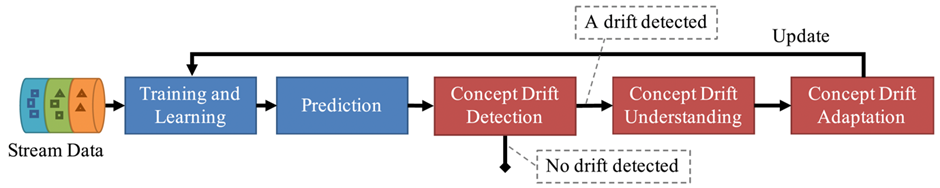
\includegraphics[width=.9\textwidth]{2_Background/figures/concept_drift_components.png}
    \caption{Main Components of Concept Drift \cite{8496795}. \\ \textcolor{gray}{\fontsize{10}{0}\selectfont DOI: 10.1109/TKDE.2018.2876857}}

    \label{fig:concept-drift-components}
\end{figure}
\vspace{-6mm}


%==============================[detection subsection]===============
\subsection{Concept Drift Detection}
Drift detection involves techniques and mechanisms to characterize and quantify concept drift by identifying change points or intervals \cite{liu2018making}. The general framework for drift detection consists of four stages:
\begin{itemize}
    \setlength{\itemsep}{0pt}
    \setlength{\parskip}{0pt}
    \item \textbf{Stage 1 (Data Retrieval):} This stage focuses on retrieving data chunks from data streams. Given that a single data instance lacks sufficient information to infer the overall distribution \cite{lu2016concept}, organizing data chunks meaningfully is crucial for effective data stream analysis \cite{ramirez2017survey}.
    \item \textbf{Stage 2 (Data Modeling):} This optional stage abstracts the retrieved data, extracting key features that contain sensitive information impacting a system in case of drift. This stage may involve dimensionality reduction or sample size reduction to meet storage and online speed requirements \cite{liu2018making}.
    \item \textbf{Stage 3 (Test Statistics Calculation):} This stage involves measuring dissimilarity or estimating distance to quantify drift severity and generate test statistics for hypothesis testing. Defining an accurate and robust dissimilarity measurement remains a challenging aspect of concept drift detection. Test statistics can also be used for clustering evaluation \cite{silva2013data} and to determine dissimilarity between sample sets \cite{dries2009adaptive}.
    \item \textbf{Stage 4 (Hypothesis Test):} This stage employs a specific hypothesis test to assess the statistical significance of the change observed in Stage 3, such as the p-value. These tests determine drift detection accuracy by establishing statistical bounds for the test statistics from Stage 3. Without Stage 4, the acquired test statistics are meaningless for drift detection, as they cannot establish the drift confidence interval. Commonly used hypothesis tests include estimating the distribution of test statistics \cite{alippi2008just, gama2004learning}, bootstrapping \cite{bu2016pdf, venkatasubramanianinformation}, the permutation test \cite{lu2016concept}, and Hoeffding's inequality-based bound identification \cite{frias2014online}.
\end{itemize}

Without Stage 1, concept drift detection can be framed as a two-sample test problem, where the objective is to determine if two sample sets come from the same distribution \cite{dries2009adaptive}. Any multivariate two-sample test can be used in Stages 2-4 for concept drift detection \cite{dries2009adaptive}. However, if distribution drift is not present in the target features, selecting the appropriate target feature becomes crucial for the performance of the learning system, presenting a significant challenge in concept drift detection \cite{yamada2013change}.

%==============================[detection Understanding]===============
\subsection{Understanding Phase}
The severity of concept drift is a key factor in selecting suitable adaptation strategies. Figure \ref{fig:concept-drift-understanding} shows that when concept drift is minimal, resulting in only slight changes to the decision boundary, incremental learning is sufficient. However, with high severity, where the decision boundary experiences substantial shifts, retraining a new model may be more effective than incrementally updating the existing one. While some researchers have emphasized the ability to quantify drift severity, this information is not widely applied in adaptation practices. The adaptation process offers three main approaches: Simple Retraining, where a new model is trained with recent data; Model Ensemble, which retains and reuses existing models for repeated concept drift; and Model Adjusting, which allows partial updates to a model as the data distribution changes.
\vspace{-3mm}
\begin{figure}[H]
    \centering
    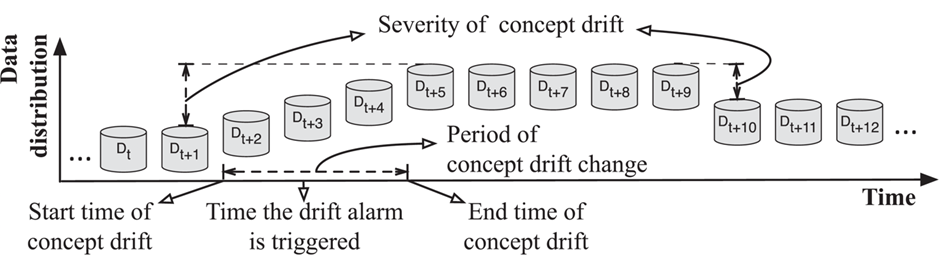
\includegraphics[width=.9\textwidth]{2_Background/figures/concept_drift_understanding.png}
    \caption{Understanding Phase of Concept Drift \cite{8496795}. \\ \textcolor{gray}{\fontsize{10}{0}\selectfont DOI: 10.1109/TKDE.2018.2876857}}
    \label{fig:concept-drift-understanding}
\end{figure}
\vspace{-6mm}

%==============================[Adaptation Adaptation]===============
\subsection{Adaptation Phase}
This section delves into strategies for updating existing learning models in response to drift, referred to as drift adaptation or reaction. The three primary categories of drift adaptation methods are simple retraining, ensemble retraining, and model adjusting, each tailored to address specific types of drift.

\begin{enumerate}[label=\Alph*.]
    \setlength{\itemsep}{0pt}
    \setlength{\parskip}{0pt}
    \item \textbf{Simple Retraining} \\
    \vspace{-3mm}

    \begin{figure}[H]
        \centering
        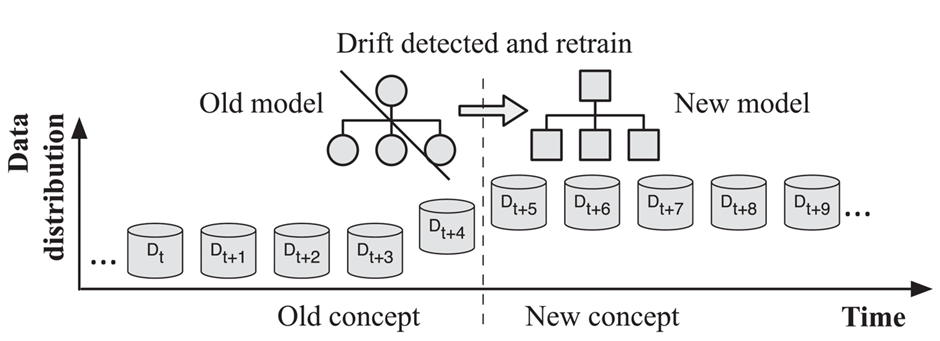
\includegraphics[width=.9\textwidth]{2_Background/figures/retrain.png}
        \caption{Approach for Retraining a New Model \cite{8496795}. \\ \textcolor{gray}{\fontsize{10}{0}\selectfont DOI: 10.1109/TKDE.2018.2876857}}
        \label{fig:concept-drift-adaptation}
    \end{figure}
    \vspace{-6mm}
    
    To handle concept drift, models can be retrained with the latest data, with a concept drift detector determining when retraining is necessary as shown in Fig. \ref{fig:concept-drift-adaptation}. A common method is the window strategy, where recent data is stored for retraining, and old data is used for drift detection. Paired Learners \cite{bach2008paired} use a stable and a reactive learner to replace the stable one when it misclassifies instances correctly classified by the reactive learner, though choosing the appropriate window size can be challenging. ADWIN \cite{bifet2007learning} improves this by dynamically adjusting window sizes based on change rates.   





\item \textbf{Model Ensemble Eetraining} \\
In recurring concept drift scenarios, ensemble methods, which reuse old models instead of retraining new ones, offer greater efficiency and adaptability \cite{sun2018concept}. These methods involve combining classifiers with varied types or parameters using voting rules. Adaptive ensemble techniques, including those based on classical methods, are designed to address concept drift challenges (Fig. \ref{fig:concept-drift-ensemble}). Classical methods like Bagging, Boosting, and Random Forests have been adapted for concept drift. Online Bagging \cite{oza2001experimental} and Bagging with ADWIN \cite{bifet2009new} replace underperforming classifiers when drift is detected. Adaptive Boosting \cite{chu2004fast} and the Adaptive Random Forest (ARF) algorithm \cite{gomes2017adaptive} also incorporate drift detection.

\vspace{-3mm}

 \begin{figure}[H]
    \centering
    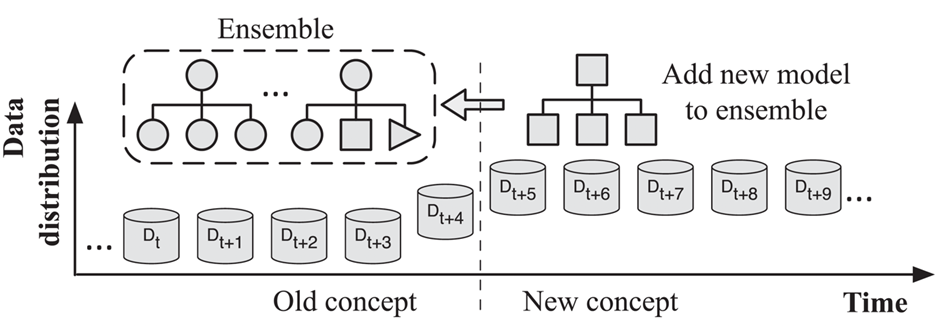
\includegraphics[width=.9\textwidth]{2_Background/figures/ensemble_update.png}
    \caption{Ensemble Approach for the Adaptation Phase \cite{8496795}. \\ \textcolor{gray}{\fontsize{10}{0}\selectfont DOI: 10.1109/TKDE.2018.2876857}}
    \label{fig:concept-drift-ensemble}
\end{figure}
\vspace{-6mm}




\item \textbf{Model Adjusting} \\
An alternative to retraining models entirely is using adaptive learning for partial updates in response to concept drift, particularly in localized regions \cite{pratama2015evolving}. Decision trees are effective due to their adaptability, with methods like VFDT \cite{domingos2000mining} using the Hoeffding bound for fast processing without storing instances. CVFDT \cite{hulten2001mining} enhances VFDT by managing concept drift with a sliding data window and replacing sub-trees for better performance. Extensions \cite{yang2012incrementally, yang2015countering} improve classifier selection with adaptive leaf strategies, while recent critiques \cite{rutkowski2012decision, rutkowski2014new} challenge VFDT's use of the Hoeffding bound and suggest alternative impurity measures.
\vspace{-3mm}

 \begin{figure}[H]
    \centering
    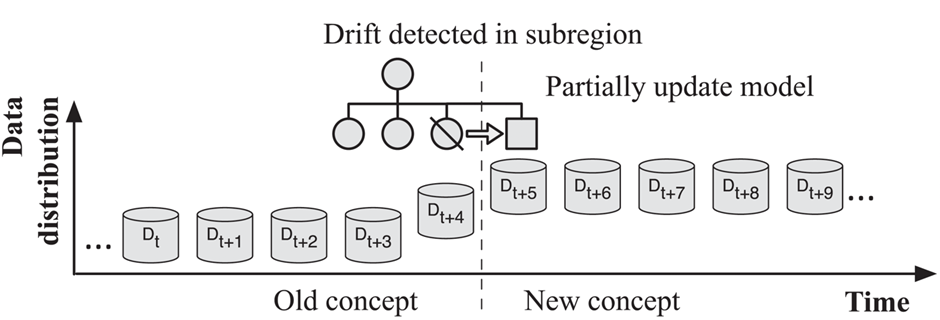
\includegraphics[width=.9\textwidth]{2_Background/figures/partial_update.png}
    \caption{Partial Updating Approach for the Adaptation Phase \cite{8496795}. \\ \textcolor{gray}{\fontsize{10}{0}\selectfont DOI: 10.1109/TKDE.2018.2876857}}
    \label{fig:concept-drift-partial-update}
\end{figure}
\vspace{-6mm}

\end{enumerate}
